% Chapter 1

\chapter{Introducción general} % Main chapter title

\label{Chapter1} % For referencing the chapter elsewhere, use \ref{Chapter1} 
\label{IntroGeneral}

%----------------------------------------------------------------------------------------

% Define some commands to keep the formatting separated from the content 
\newcommand{\keyword}[1]{\textbf{#1}}
\newcommand{\tabhead}[1]{\textbf{#1}}
\newcommand{\code}[1]{\texttt{#1}}
\newcommand{\file}[1]{\texttt{\bfseries#1}}
\newcommand{\option}[1]{\texttt{\itshape#1}}
\newcommand{\grados}{$^{\circ}$}

%----------------------------------------------------------------------------------------

%\section{Introducción}

%----------------------------------------------------------------------------------------

% Párrafo introductorio al capítulo 1
En este apartado se introducen los conceptos básicos sobre el dispositivo de adquisición de señales neurofisiológicas, sobre su estado del arte, sobre el marco normativo aplicado, y sobre la motivación, objetivos y alcance para llevar adelante este trabajo.

\section{Dispositivo de adquisición de señales neurofisiológicas}

El dispositivo de adquisición de señales neurofisiológicas (DASN), es un módulo de hardware y software embebido destinado a ser parte de un sistema electro-médico.
El desarrollo está enmarcado en una serie de proyectos de investigación del Grupo de Tecnología en Neuroseñales de la Universidad Nacional de La Matanza (GTN UNLAM) cuya finalidad es generar una plataforma de uso común para fabricantes locales, para investigación en las universidades y para el eventual desarrollo de nuevos productos y empresas de tecnología médica. 

En la Figura \ref{fig:diagBloquesSistema} se puede ver un diagrama en bloques de un sistema electromédico que incorpora al módulo DASN. Forman parte también del sistema un estimulador que interactúa con el paciente y un equipo de registro donde se guardan en formato digital los biopotenciales del paciente. Tanto el estimulador como el equipo de registro se comunican con el módulo DASN cuya función es adquirir señales eléctricas provenientes del sistema nervioso del paciente.

\vspace{1cm}

\begin{figure}[htbp]
	\centering
	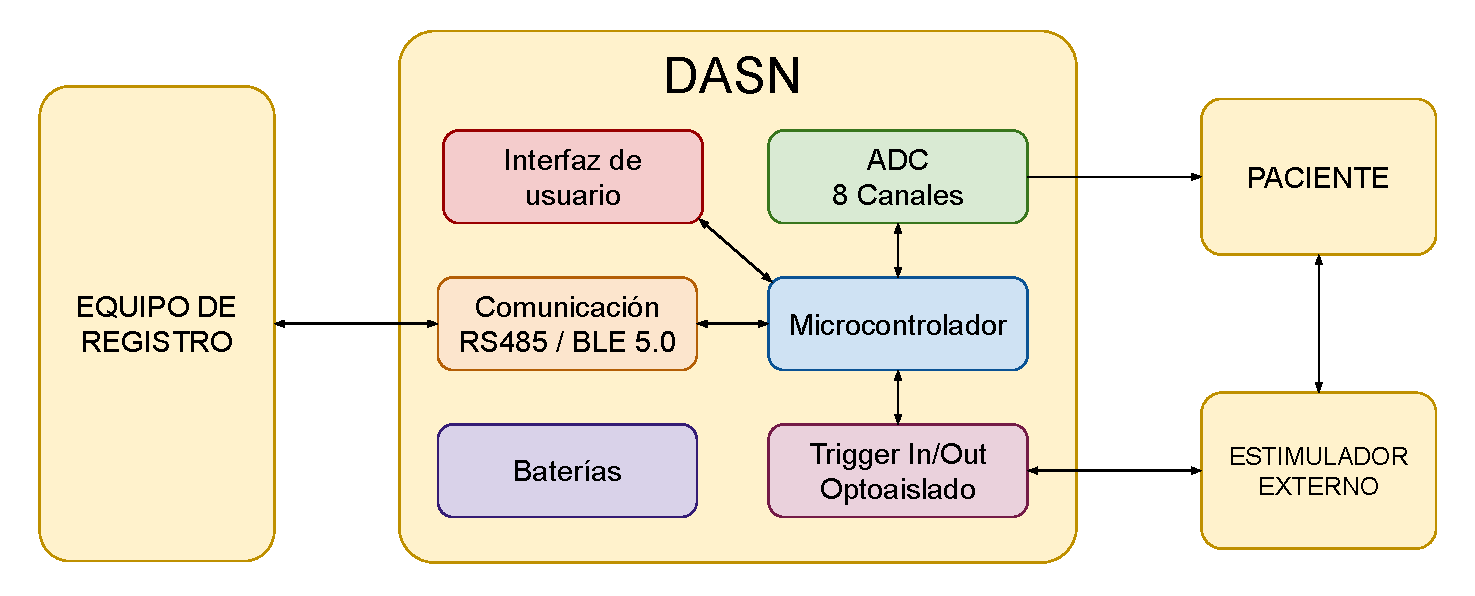
\includegraphics[width=1\textwidth]{./Figures/DiagramaEnBloquesDASN.pdf}
	\caption{Diagrama en bloques del sistema.}
	\label{fig:diagBloquesSistema}
\end{figure}

\vspace{1cm}

El DASN tiene 8 canales de entrada, comunicación inalámbrica a través de una comunicación bluetooth, y cableada a través de una comunicación RS485. Las señales adquiridas se pueden sincronizar con el estimulador externo, pudiendo funcionar como master o slave. Tiene la posibilidad de alimentarse por baterías y posee una interfaz de usuario para dar indicaciones de encendido, apagado y estado de funcionamiento.

\section{Estado del arte}
En particular para el subsector de la Neurofisiología, no existen placas comerciales que cumplan con las condiciones aplicables a un equipamiento médico de registro de señales neurofisiológicas. Si existen algunos ejemplos de placas de uso recreacional, didáctico o comercial, con un principio de funcionamiento similar pero destinado a interfaces cerebro-máquina (BCI). Ninguna de estas placas está destinada a la aplicación directa a la tecnología médica, ni posee certificaciones de calidad, ni garantiza características de funcionamiento esencial ni de seguridad básica.

\section{Marco normativo}
Las regulaciones de los dispositivos médicos tienen como objetivo proteger la salud de los pacientes, usuarios y terceros. Intentan asegurar la seguridad y eficacia de los productos disponibles en el mercado. Para cumplir con dichas regulaciones se debe actuar bajo las normas que son aceptadas por los organismos de control de los estados. Normas sobre sistemas de gestión de la calidad, sobre procesos y sobre productos alcanzan al diseño y la producción de equipamiento médico, incluido el software que lo conforma. La norma IEC 62304 \citep{REF} define las condiciones que debe cumplir el ciclo de vida del software; es decir, se trata de una norma de proceso. La IEC 60601-1 \citep{REF} (cuyo punto 14 se encarga del software del producto electro-médico o PEMS) y la IEC 82304-1 \citep{REF} son normas que definen las características que debe cumplir el software para que sea seguro y eficaz. La IEC 62304 no impone o prohíbe una metodología de desarrollo de software en particular, pero sí indica cuales son las características que debe tener el proceso de ciclo de vida elegido. Debe tratarse de un proceso controlado, que tenga en cuenta la verificación y validación del software durante el proceso de desarrollo, que provea evidencia documentada para demostrar el cumplimiento del proceso, que responda a una planificación, que tome en cuenta el análisis de los riesgos relacionados con el producto, entre otras consideraciones más. La norma no entra en detalle de cómo esas actividades deben ser ejecutadas, dejando al fabricante la libertad de crear sus propias prácticas para que sean coherentes con los principios regulatorios.

\section{Motivación}
La Neurofisiología es una rama de las neurociencias, que se encarga del estudio funcional de la actividad bioeléctrica del sistema nervioso central, periférico y autonómico, mediante la utilización de equipos y técnicas de análisis avanzado, como la Electroencefalografía (EEG), la Electromiografía (EMG), los Potenciales Evocados (PE), la Polisomnografía (PSG) y otras nuevas técnicas como el neuromonitoreo (NM) o la medición de profundidad de anestesia (MPA). La plataforma de adquisición de señales neurofisiológicas está pensada para cubrir las necesidades de fabricantes de equipos del subsector de las neurociencias, para la investigación en las universidades y para el eventual desarrollo de nuevos productos y empresas de tecnología médica. En este marco nació la propuesta para dar vida al primer prototipo mediante la programación de su sistema embebido, con la motivación de aportar a la soberanía tecnológica y a la mejora del sistema de salud. 

\section{Objetivos y alcance}
\subsection{Objetivos del trabajo}

El objetivo del presente trabajo final de carrera fue diseñar, implementar, ensayar y documentar la primera versión funcional del software embebido del DASN de acuerdo a los lineamientos impartidos en las distintas materias de la Especialización en Sistemas Embebidos de la Universidad de Buenos Aires.

\subsection{Alcances del trabajo}
El presente trabajo incluye:
\begin{itemize}
\item Diseño del software embebido del DASN.
\item Diseño del protocolo de comunicación entre DASN y equipo de registro.
\item Software de prueba para simular un equipo de registro y probar el DASN.
\end{itemize}

El presente trabajo no incluye:
\begin{itemize}
\item Diseño de hardware.
\item Filtrado digital de las señales adquiridas.
\item Validación de la norma ISO 62304.
\end{itemize}

